% --------------------------
% Document class
% --------------------------
\documentclass[
A4paper,            1 paper size A4
oneside,            % oneside or twoside printing
openright,          % doublepage cleaning ends up right side
10pt,               % font size
headings=normal,    % size of headings
titlepage=on        % own page for each title page
]{article}
% **************************************************
% THESIS details
% **************************************************
\newcommand{\University}{\protect{Universidad Polit\'ecnica de Madrid}}
\newcommand{\UNIVERSITY}{\protect{UNIVERSIDAD POLIT\'ECNICA DE MADRID}}
\newcommand{\thesisTitle}{\protect {Entrega final Sistemas no Lineales}}
\newcommand{\thesisDate}{\today}
\newcommand{\UPMCentre}{\protect {Escuela Técnica Superior de Ingenieros Industriales}}

\newcommand\blankpage{%
    \null
    \thispagestyle{empty}%
    \addtocounter{page}{-1}%
    \newpage}
\renewcommand{\familydefault}{\sfdefault}
% **************************************************
% Settings
% **************************************************
% This line pulls in all your packages and biblatex settings

\input{settings} 
\usepackage[numbers,sort&compress]{natbib}
\bibliographystyle{IEEEtran}




\usepackage[table]{xcolor}
\usepackage{colortbl}
\definecolor{gris}{RGB}{242,242,242}

% TikZ packages for diagrams
\usepackage{tikz}
\usetikzlibrary{calc,arrows.meta,decorations.pathmorphing,patterns,angles,quotes}
\usepackage{pgfplots}
\pgfplotsset{compat=1.18}

% **************************************************
% Begin document
% **************************************************

\begin{document}

% --------------------------
% Cover
% --------------------------

\pagestyle{empty}                % no header nor footer
\input{cover}  
\newpage
\selectlanguage{english}
\setcounter{tocdepth}{3}        % define depth of toc
\tableofcontents                % display table of contents
\clearpage

% --------------------------
% Main matter
% --------------------------
\pagenumbering{arabic}
\setcounter{page}{1}
\pagestyle{fancy}

\section{Introducción}
El objetivo del proyecto es automatizar el juego de la recreativa Monza, un sistema dinámico altamente no lineal. El juego consiste en guiar una moneda a través de múltiples niveles de rieles con forma parabólica rotando el tablero completo mediante un actuador angular $\theta$.



% PLACEHOLDER: Imagen de la máquina real o esquema general
\begin{figure}[H]
    \centering
    % \includegraphics[width=0.6\textwidth]{ruta/a/imagen_maquina_real.png}
    \fbox{\begin{minipage}{0.6\textwidth}
        \centering
        \vspace{1cm}
        \textbf{[INSERTAR IMAGEN: Foto de la recreativa Monza]}
        \vspace{1cm}
    \end{minipage}}
    \caption{Niveles de dificultad de la recreativa Monza y disposición de los rieles.}
    \label{fig:niveles}
\end{figure}

\section{Modelado Matemático del Sistema}
Para simular el comportamiento de la moneda, se han derivado las ecuaciones físicas que rigen su movimiento en las distintas fases del juego.

\subsection{Geometría del Tablero}
Los rieles se modelan como parábolas desfasadas verticalmente. La ecuación general en el sistema de referencia del tablero $(x_1, y_1)$ es:
\begin{equation}
    y_1 = -0.54 \cdot x_1^2 + C
\end{equation}
Donde $C$ varía según el nivel del piso. El ángulo de inclinación local $\phi(x)$ se determina mediante la derivada de la curva. La pendiente local se calcula numéricamente mediante:
\begin{equation}
    \text{slope}(x) = \frac{\nabla y(x)}{\nabla x(x)}
\end{equation}
donde $\nabla$ representa el operador gradiente discreto. El ángulo de inclinación local se obtiene como:
\begin{equation}
    \alpha(x) = \arctan(\text{slope}(x))
\end{equation}



\begin{figure}[H]
    \centering
    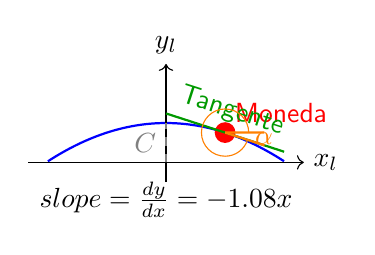
\begin{tikzpicture}[scale=2.5]
        % Draw parabola y = -0.54*x^2 + 0.2
        \draw[thick, blue] plot[smooth, domain=-0.6:0.6, samples=100] (\x, {-0.54*\x*\x + 0.2});
        
        % Draw coordinate axes
        \draw[->] (-0.7,0) -- (0.7,0) node[right] {$x_l$};
        \draw[->] (0,-0.1) -- (0,0.5) node[above] {$y_l$};
        
        % Mark a point on the parabola
        \coordinate (P) at (0.3, {-0.54*0.3*0.3 + 0.2});
        \fill[red] (P) circle (1.5pt) node[above right] {Moneda};
        
        % Draw tangent line at point P
        \draw[green!60!black, thick] ($(P) + (-0.3, {-0.54*2*0.3*(-0.3)})$) -- 
                                     ($(P) + (0.3, {-0.54*2*0.3*0.3})$) 
                                     node[midway, above, sloped] {Tangente};
        
        % Draw angle alpha
        \coordinate (P1) at ($(P) + (0.2, 0)$);
        \coordinate (P2) at ($(P) + (0.2, {-0.54*2*0.3*0.2})$);
        \draw[orange, thick] (P) -- (P1);
        \draw[orange, thick] (P) -- (P2) node[midway, right] {$\alpha$};
        \pic[draw=orange, angle radius=0.3cm, angle eccentricity=1.3] {angle={P1--P--P2}};
        
        % Label slope
        \node[below] at (0, -0.05) {$\text{slope} = \frac{dy}{dx} = -1.08x$};
        
        % Draw vertical offset indicator
        \draw[dashed, gray] (0,0) -- (0,0.2) node[midway, left] {$C$};
    \end{tikzpicture}
    \caption{Parámetros geométricos de las parábolas que conforman los rieles.}
    \label{fig:geometria}
\end{figure}

\subsection{Dinámica del Movimiento en el Carril}
El movimiento de la moneda considera fuerzas de gravedad, fricción viscosa con el aire, rozamiento con el carril y contacto con la pared lateral.

Se distinguen dos modos de movimiento:
\begin{itemize}
    \item \textbf{Deslizamiento puro:} Cuando la fricción es insuficiente para generar rodadura.
    \item \textbf{Rodadura sin deslizamiento:} Condición regida por el coeficiente de fricción estática $\mu_s$.
\end{itemize}

Las ecuaciones dinámicas en el sistema no inercial incluyen la fuerza centrífuga y de Coriolis debido a la rotación $\theta$ del tablero.

\subsubsection{Transformaciones de Coordenadas}
Para transformar entre el sistema de coordenadas local del tablero $(x_l, y_l)$ y el sistema global $(x_g, y_g)$, se utilizan las siguientes rotaciones:

\begin{equation}
    \begin{bmatrix} x_g \\ y_g \end{bmatrix} = \begin{bmatrix} \cos\theta & -\sin\theta \\ \sin\theta & \cos\theta \end{bmatrix} \begin{bmatrix} x_l \\ y_l \end{bmatrix}
\end{equation}

La transformación inversa (global a local) viene dada por:
\begin{equation}
    \begin{bmatrix} x_l \\ y_l \end{bmatrix} = \begin{bmatrix} \cos\theta & \sin\theta \\ -\sin\theta & \cos\theta \end{bmatrix} \begin{bmatrix} x_g \\ y_g \end{bmatrix}
\end{equation}

\begin{figure}[H]
    \centering
    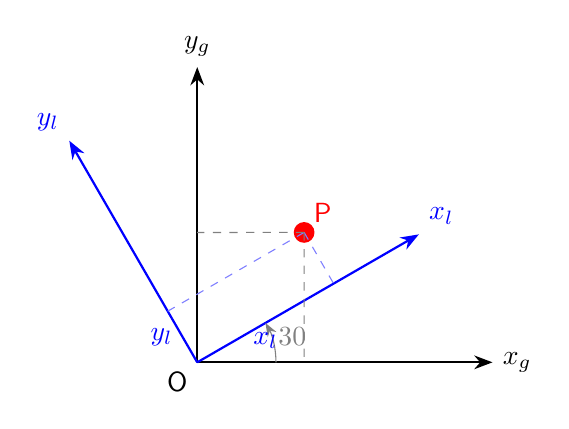
\begin{tikzpicture}[scale=2.5, >=Stealth]
        % Global coordinate system
        \draw[->, thick, black] (0,0) -- (1.5,0) node[right] {$x_g$};
        \draw[->, thick, black] (0,0) -- (0,1.5) node[above] {$y_g$};
        \node[below left] at (0,0) {O};
        
        % Local coordinate system (rotated by theta)
        \def\theta{30}
        \draw[->, thick, blue] (0,0) -- ({1.3*cos(\theta)}, {1.3*sin(\theta)}) 
            node[above right] {$x_l$};
        \draw[->, thick, blue] (0,0) -- ({-1.3*sin(\theta)}, {1.3*cos(\theta)}) 
            node[above left] {$y_l$};
        
        % Draw angle arc
        \draw[->, gray] (0.4,0) arc (0:\theta:0.4);
        \node[gray] at ({0.5*cos(\theta/2)}, {0.5*sin(\theta/2)}) {$\theta$};
        
        % Example point in local coordinates
        \coordinate (P) at ({0.8*cos(\theta) - 0.3*sin(\theta)}, {0.8*sin(\theta) + 0.3*cos(\theta)});
        \fill[red] (P) circle (1.5pt) node[above right] {P};
        
        % Projections to local axes
        \draw[dashed, blue!50] (P) -- ({0.8*cos(\theta)}, {0.8*sin(\theta)});
        \draw[dashed, blue!50] (P) -- ({-0.3*sin(\theta)}, {0.3*cos(\theta)});
        
        % Projections to global axes
        \draw[dashed, black!50] (P) -- ({0.8*cos(\theta) - 0.3*sin(\theta)}, 0);
        \draw[dashed, black!50] (P) -- (0, {0.8*sin(\theta) + 0.3*cos(\theta)});
        
        % Labels
        \node[blue] at ({0.4*cos(\theta)}, {0.4*sin(\theta)}) [below] {$x_l$};
        \node[blue] at ({-0.15*sin(\theta)}, {0.15*cos(\theta)}) [left] {$y_l$};
    \end{tikzpicture}
    \caption{Transformación de coordenadas entre el sistema local (rotado) y el sistema global.}
    \label{fig:coordenadas}
\end{figure}

\subsubsection{Ecuaciones de Movimiento en el Carril}
Durante el movimiento de rodadura, la aceleración tangencial local se calcula como:
\begin{equation}
    a_l = -g \sin(\alpha + \theta) - \mu_v v_l
\end{equation}
donde $g$ es la aceleración gravitatoria, $\alpha$ es el ángulo de inclinación local del riel, $\theta$ es el ángulo de rotación del tablero, $\mu_v$ es el coeficiente de fricción viscosa y $v_l$ es la velocidad local tangencial.

La integración temporal se realiza mediante el método de Euler:
\begin{align}
    v_l(t+\Delta t) &= v_l(t) + a_l(t) \Delta t \\
    x_l(t+\Delta t) &= x_l(t) + v_l(t) \Delta t \\
    y_l(t+\Delta t) &= f(x_l(t+\Delta t))
\end{align}
donde $f(x)$ es la función que describe la geometría del riel (interpolación cúbica de los puntos discretos).



\begin{figure}[H]
    \centering
    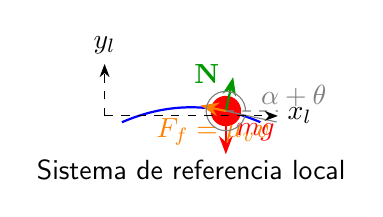
\begin{tikzpicture}[scale=2.2, >=Stealth]
        % Draw track segment
        \draw[thick, blue] plot[smooth, domain=-0.4:0.4, samples=50] 
            (\x, {-0.54*\x*\x + 0.15});
        
        % Ball position
        \coordinate (ball) at (0.2, {-0.54*0.2*0.2 + 0.15});
        \fill[red] (ball) circle (2.5pt);
        
        % Calculate slope at ball position
        \def\slope{-0.54*2*0.2}
        \def\angle{atan(\slope)}
        
        % Draw forces
        % Weight (mg) - vertical downward
        \draw[->, thick, red] (ball) -- ($(ball) + (0, -0.25)$) 
            node[midway, right] {$mg$};
        
        % Normal force - perpendicular to track
        \draw[->, thick, green!60!black] (ball) -- 
            ($(ball) + ({0.2*cos(\angle + 90)}, {0.2*sin(\angle + 90)})$) 
            node[midway, above left] {$\mathbf{N}$};
        
        % Friction force - along track opposite to velocity
        \draw[->, thick, orange] (ball) -- 
            ($(ball) + ({-0.15*cos(\angle)}, {-0.15*sin(\angle)})$) 
            node[midway, below] {$F_f = \mu_v v$};
        
        % Draw angle indicators
        \coordinate (ball_h) at ($(ball) + (0.3, 0)$);
        \coordinate (ball_slope) at ($(ball) + ({0.3*cos(\angle)}, {0.3*sin(\angle)})$);
        \draw[dashed, gray] (ball) -- (ball_h);
        \draw[gray] (ball) -- (ball_slope) 
            node[midway, above right] {$\alpha + \theta$};
        \pic[draw=gray, angle radius=0.25cm] 
            {angle={ball_h--ball--ball_slope}};
        
        % Coordinate system
        \draw[->, dashed, thin] (-0.5, 0.1) -- (0.5, 0.1) node[right] {$x_l$};
        \draw[->, dashed, thin] (-0.5, 0.1) -- (-0.5, 0.4) node[above] {$y_l$};
        
        % Label
        \node[below] at (0, -0.1) {Sistema de referencia local};
    \end{tikzpicture}
    \caption{Diagrama de cuerpo libre de la moneda sobre el riel parabólico.}
    \label{fig:fuerzas}
\end{figure}

\subsection{Modelado de Caída y Rebote}
Cuando la moneda abandona un riel, entra en una fase de caída libre hasta impactar con el siguiente nivel. El impacto se modela como un choque inelástico caracterizado por un coeficiente de restitución $k$, perdiendo energía en cada rebote.

\subsubsection{Transición de Rodadura a Caída Libre}
Al abandonar un riel, la velocidad global se calcula combinando la velocidad local transformada y la velocidad tangencial debida a la rotación del tablero:
\begin{align}
    v_{x,\text{loc}} &= v_l \\
    v_{y,\text{loc}} &= \text{slope} \cdot v_l \\
    \begin{bmatrix} v_{x,\text{rel}} \\ v_{y,\text{rel}} \end{bmatrix} &= \begin{bmatrix} \cos\theta & -\sin\theta \\ \sin\theta & \cos\theta \end{bmatrix} \begin{bmatrix} v_{x,\text{loc}} \\ v_{y,\text{loc}} \end{bmatrix} \\
    v_{x,\text{tan}} &= -\dot{\theta} \cdot y_g \\
    v_{y,\text{tan}} &= \dot{\theta} \cdot x_g
\end{align}
La velocidad global inicial de caída es:
\begin{equation}
    \begin{bmatrix} v_{x,g} \\ v_{y,g} \end{bmatrix} = \begin{bmatrix} v_{x,\text{rel}} \\ v_{y,\text{rel}} \end{bmatrix} + \begin{bmatrix} v_{x,\text{tan}} \\ v_{y,\text{tan}} \end{bmatrix}
\end{equation}

\subsubsection{Dinámica de Caída Libre}
Durante la caída, el movimiento se rige por:
\begin{align}
    v_{y,g}(t+\Delta t) &= v_{y,g}(t) - g \Delta t \\
    x_g(t+\Delta t) &= x_g(t) + v_{x,g}(t) \Delta t \\
    y_g(t+\Delta t) &= y_g(t) + v_{y,g}(t) \Delta t
\end{align}

\subsubsection{Resolución de Colisiones}
Al detectar una colisión con un riel, se calcula el vector normal a la superficie:
\begin{align}
    \phi &= \arctan(\text{slope}) + \theta \\
    \mathbf{n} &= \begin{bmatrix} -\sin\phi \\ \cos\phi \end{bmatrix}
\end{align}

La componente normal de la velocidad es:
\begin{equation}
    v_n = \mathbf{v}_g \cdot \mathbf{n} = v_{x,g} n_x + v_{y,g} n_y
\end{equation}

El impulso de rebote se calcula mediante:
\begin{equation}
    J = -(1 + k) v_n
\end{equation}
donde $k$ es el coeficiente de restitución. La velocidad después del impacto es:
\begin{equation}
    \begin{bmatrix} v_{x,g}' \\ v_{y,g}' \end{bmatrix} = \begin{bmatrix} v_{x,g} \\ v_{y,g} \end{bmatrix} + J \mathbf{n}
\end{equation}

Si la velocidad normal de impacto es suficientemente pequeña ($|v_n| < 0.5$ m/s), la moneda se adhiere al riel y retorna al estado de rodadura, proyectando la velocidad global sobre la tangente local:
\begin{equation}
    v_l = \mathbf{v}_g' \cdot \mathbf{t} = v_{x,g}' \cos\phi + v_{y,g}' \sin\phi
\end{equation}
donde $\mathbf{t} = [\cos\phi, \sin\phi]^T$ es el vector tangente unitario.

\section{Identificación de Parámetros}
Los parámetros físicos del modelo han sido ajustados experimentalmente para coincidir con el comportamiento de la caja negra de Simulink. La Tabla~\ref{tab:parametros} muestra los valores utilizados en la implementación del código Python.

\begin{table}[H]
    \centering
    \caption{Parámetros del modelo físico utilizados en la simulación.}
    \label{tab:parametros}
    \begin{tabular}{lcc}
        \toprule
        \textbf{Parámetro} & \textbf{Símbolo} & \textbf{Valor} \\
        \midrule
        Gravedad & $g$ & 9.81 m/s$^2$ \\
        Coef. fricción viscosa & $\mu_v$ & 0.01 \\
        Coef. restitución choque & $k$ & 0.1 \\
        Paso temporal (física) & $\Delta t$ & 0.033 s \\
        Sub-pasos físicos & $n_{\text{sub}}$ & 10 \\
        Paso temporal interno & $\delta t = \Delta t/n_{\text{sub}}$ & 0.0033 s \\
        Ángulo máximo de inclinación & $\theta_{\max}$ & 45$^\circ$ (0.785 rad) \\
        Velocidad angular máxima & $\omega_{\max}$ & 8.0 rad/s \\
        Setpoint de posición & $x_{\text{sp}}$ & 0.0 m \\
        Duración de simulación & $T$ & 2.0 s \\
        \bottomrule
    \end{tabular}
\end{table}

Los parámetros físicos fundamentales son la gravedad $g = 9.81$ m/s$^2$, el coeficiente de fricción viscosa $\mu_v = 0.01$ que modela la resistencia al movimiento, y el coeficiente de restitución $k = 0.1$ que determina la pérdida de energía en los choques. El paso temporal de simulación $\Delta t = 0.033$ s corresponde a una frecuencia de muestreo de aproximadamente 30 Hz, mientras que internamente se utilizan $n_{\text{sub}} = 10$ sub-pasos para mayor precisión en la integración numérica, resultando en un paso temporal interno de $\delta t = 0.0033$ s.

Para el control del sistema, se establece un límite máximo de inclinación del tablero de $\theta_{\max} = 45^\circ$ y una velocidad angular máxima de $\omega_{\max} = 8.0$ rad/s para evitar movimientos bruscos. El setpoint de posición se fija en $x_{\text{sp}} = 0.0$ m, correspondiente al centro del tablero.

\begin{figure}[H]
    \centering
    \includegraphics[width=0.6\textwidth]{figures/comparacion.png}
    
    \caption{Comparación de trayectorias entre modelo de simulink y modelo propio desde el punto inicial con un ángulo de -0.12 rad.}
    \label{fig:trayectoria}
\end{figure}

\section{Estrategias de Control Implementadas}
Se han diseñado e implementado controladores para gobernar el ángulo $\theta$ del tablero y asegurar que la moneda complete el recorrido.

\subsection{Control por Modos Deslizantes (SMC)}
El controlador SMC busca llevar el estado del sistema a una superficie de deslizamiento $s(t) = 0$. Se definen las variables de error $e$ (posición respecto al objetivo) y $\dot{e}$.
\begin{equation}
    s(t) = e(t) + \lambda \cdot \dot{e}(t)
\end{equation}
La ley de control aplicada es del tipo conmutada:
\begin{equation}
    u = -k \cdot \text{sign}(s(t))
\end{equation}



\begin{figure}[H]
    \centering
    \begin{tikzpicture}[scale=1.8, >=Stealth]
        % Draw axes
        \draw[->] (-2.5,0) -- (2.5,0) node[right] {$e$};
        \draw[->] (0,-2.5) -- (0,2.5) node[above] {$\dot{e}$};
        
        % Draw sliding surface s = e + lambda*e_dot = 0
        \def\lambda{0.5}
        \draw[thick, blue] (-2.5, {2.5/\lambda}) -- (2.5, {-2.5/\lambda}) 
            node[above right] {$s = e + \lambda\dot{e} = 0$};
        
        % Draw region labels
        \node[blue!50] at (-1.5, 1.5) {$s > 0$};
        \node[blue!50] at (1.5, -1.5) {$s < 0$};
        
        % Draw trajectory approaching sliding surface
        \draw[thick, red, ->] (-2, 2) .. controls (-1, 1.5) and (-0.5, 0.8) .. 
            (-0.3, 0.3) .. controls (-0.1, 0.1) .. (0, 0);
        \draw[thick, red, ->] (2, -2) .. controls (1, -1.5) and (0.5, -0.8) .. 
            (0.3, -0.3) .. controls (0.1, -0.1) .. (0, 0);
        
        % Mark origin
        \fill[black] (0,0) circle (1.5pt) node[below left] {Origen};
        
        % Draw reaching phase arrows
        \draw[->, green!60!black, thick] (-1.8, 1.8) -- (-1.2, 1.2) 
            node[midway, above left] {Fase de alcance};
        \draw[->, green!60!black, thick] (1.8, -1.8) -- (1.2, -1.2) 
            node[midway, below right] {Fase de alcance};
        
        % Draw sliding phase
        \draw[->, orange, thick] (-0.5, 0.25) -- (0, 0) 
            node[midway, above] {Fase de deslizamiento};
        
        % Add grid
        \draw[gray!30, very thin] (-2.5,-2.5) grid (2.5,2.5);
    \end{tikzpicture}
    \caption{Trayectoria en el espacio de estados hacia la superficie de deslizamiento.}
    \label{fig:smc}
\end{figure}

\subsection{Control de Lógica Difusa (Fuzzy Logic)}
Se implementó un controlador tipo Mamdani basado en reglas heurísticas.
\begin{itemize}
    \item \textbf{Entradas:} Error de posición $e = x_{\text{setpoint}} - x_g$ y Velocidad global $v_{x,g}$ de la moneda.
    \item \textbf{Salida:} Ángulo objetivo $\theta_{\text{target}}$ del tablero.
    \item \textbf{Funciones de Pertenencia:} Triangulares para cinco conjuntos: NB (Negative Big), NS (Negative Small), Z (Zero), PS (Positive Small), PB (Positive Big).
\end{itemize}

\subsubsection{Funciones de Pertenencia Triangulares}
La función de pertenencia triangular se define como:
\begin{equation}
    \mu(x; a, b, c) = \max\left(0, \min\left(\frac{x-a}{b-a}, \frac{c-x}{c-b}\right)\right)
\end{equation}
donde $a$, $b$ y $c$ son los vértices izquierdo, central y derecho del triángulo, respectivamente.

Los centros de los conjuntos difusos para las entradas son:
\begin{align}
    \mathcal{E} &= \{-0.5, -0.25, 0.0, 0.25, 0.5\} \quad \text{(Error)} \\
    \mathcal{V} &= \{-1.0, -0.75, 0.0, 0.75, 1.0\} \quad \text{(Velocidad)} \\
    \mathcal{U} &= \{-1, -0.75, 0.0, 0.75, 1\} \quad \text{(Salida, normalizada)}
\end{align}

\subsubsection{Evaluación de Reglas y Defuzzificación}
Para cada regla $R_i: \text{IF } e \text{ is } E_i \text{ AND } v \text{ is } V_i \text{ THEN } u \text{ is } U_i$, la fuerza de activación se calcula mediante el operador mínimo:
\begin{equation}
    w_i = \min(\mu_E(e), \mu_V(v))
\end{equation}

La salida defuzzificada se obtiene mediante el método del centroide (promedio ponderado):
\begin{equation}
    u = \frac{\sum_{i=1}^{N} w_i \cdot c_i}{\sum_{i=1}^{N} w_i}
\end{equation}
donde $c_i$ es el centro del conjunto difuso de salida $U_i$ y $N$ es el número de reglas activas. Si $\sum w_i = 0$, la salida es $u = 0$.

El ángulo objetivo del tablero se calcula como:
\begin{equation}
    \theta_{\text{target}} = \text{clip}(-u, -\theta_{\max}, \theta_{\max})
\end{equation}
donde $\theta_{\max} = 45°$ es el límite máximo de inclinación.

\subsubsection{Cinemática del Actuador}
El controlador limita la velocidad angular del actuador mediante:
\begin{equation}
    \omega = \text{clip}\left(\frac{\theta_{\text{target}} - \theta}{\Delta t}, -\omega_{\max}, \omega_{\max}\right)
\end{equation}
donde $\omega_{\max} = 8$ rad/s. La actualización del ángulo se realiza mediante integración de Euler:
\begin{equation}
    \theta(t+\Delta t) = \theta(t) + \omega \Delta t
\end{equation}



\begin{figure}[H]
    \centering
    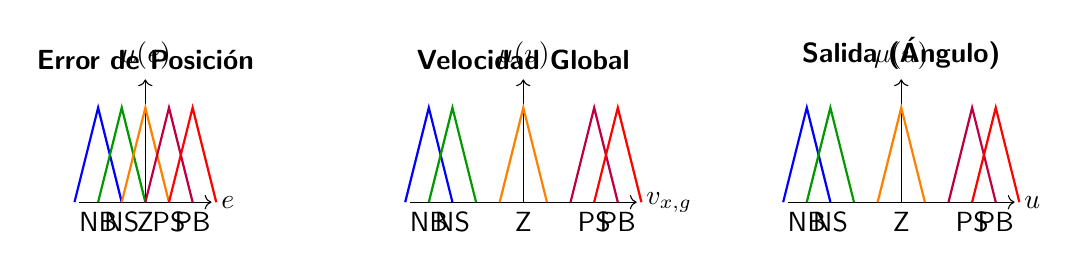
\begin{tikzpicture}[scale=1.2]
        % Error membership functions
        \begin{scope}[xshift=0cm]
            \draw[->] (-0.7,0) -- (0.7,0) node[right] {$e$};
            \draw[->] (0,0) -- (0,1.3) node[above] {$\mu(e)$};
            
            % Define centers
            \def\nb{-0.5}
            \def\ns{-0.25}
            \def\z{0.0}
            \def\ps{0.25}
            \def\pb{0.5}
            
            % NB triangle
            \draw[thick, blue] (\nb-0.25,0) -- (\nb,1) -- (\nb+0.25,0);
            \node[below] at (\nb, 0) {NB};
            
            % NS triangle
            \draw[thick, green!60!black] (\ns-0.25,0) -- (\ns,1) -- (\ns+0.25,0);
            \node[below] at (\ns, 0) {NS};
            
            % Z triangle
            \draw[thick, orange] (\z-0.25,0) -- (\z,1) -- (\z+0.25,0);
            \node[below] at (\z, 0) {Z};
            
            % PS triangle
            \draw[thick, purple] (\ps-0.25,0) -- (\ps,1) -- (\ps+0.25,0);
            \node[below] at (\ps, 0) {PS};
            
            % PB triangle
            \draw[thick, red] (\pb-0.25,0) -- (\pb,1) -- (\pb+0.25,0);
            \node[below] at (\pb, 0) {PB};
            
            \node[above] at (0, 1.3) {\textbf{Error de Posición}};
        \end{scope}
        
        % Velocity membership functions
        \begin{scope}[xshift=4cm]
            \draw[->] (-1.2,0) -- (1.2,0) node[right] {$v_{x,g}$};
            \draw[->] (0,0) -- (0,1.3) node[above] {$\mu(v)$};
            
            % Define centers
            \def\nb{-1.0}
            \def\ns{-0.75}
            \def\z{0.0}
            \def\ps{0.75}
            \def\pb{1.0}
            
            % NB triangle
            \draw[thick, blue] (\nb-0.25,0) -- (\nb,1) -- (\nb+0.25,0);
            \node[below] at (\nb, 0) {NB};
            
            % NS triangle
            \draw[thick, green!60!black] (\ns-0.25,0) -- (\ns,1) -- (\ns+0.25,0);
            \node[below] at (\ns, 0) {NS};
            
            % Z triangle
            \draw[thick, orange] (\z-0.25,0) -- (\z,1) -- (\z+0.25,0);
            \node[below] at (\z, 0) {Z};
            
            % PS triangle
            \draw[thick, purple] (\ps-0.25,0) -- (\ps,1) -- (\ps+0.25,0);
            \node[below] at (\ps, 0) {PS};
            
            % PB triangle
            \draw[thick, red] (\pb-0.25,0) -- (\pb,1) -- (\pb+0.25,0);
            \node[below] at (\pb, 0) {PB};
            
            \node[above] at (0, 1.3) {\textbf{Velocidad Global}};
        \end{scope}
        
        % Output membership functions
        \begin{scope}[xshift=8cm]
            \draw[->] (-1.2,0) -- (1.2,0) node[right] {$u$};
            \draw[->] (0,0) -- (0,1.3) node[above] {$\mu(u)$};
            
            % Define centers
            \def\nb{-1.0}
            \def\ns{-0.75}
            \def\z{0.0}
            \def\ps{0.75}
            \def\pb{1.0}
            
            % NB triangle
            \draw[thick, blue] (\nb-0.25,0) -- (\nb,1) -- (\nb+0.25,0);
            \node[below] at (\nb, 0) {NB};
            
            % NS triangle
            \draw[thick, green!60!black] (\ns-0.25,0) -- (\ns,1) -- (\ns+0.25,0);
            \node[below] at (\ns, 0) {NS};
            
            % Z triangle
            \draw[thick, orange] (\z-0.25,0) -- (\z,1) -- (\z+0.25,0);
            \node[below] at (\z, 0) {Z};
            
            % PS triangle
            \draw[thick, purple] (\ps-0.25,0) -- (\ps,1) -- (\ps+0.25,0);
            \node[below] at (\ps, 0) {PS};
            
            % PB triangle
            \draw[thick, red] (\pb-0.25,0) -- (\pb,1) -- (\pb+0.25,0);
            \node[below] at (\pb, 0) {PB};
            
            \node[above] at (0, 1.3) {\textbf{Salida (Ángulo)}};
        \end{scope}
    \end{tikzpicture}
    \caption{Funciones de pertenencia triangulares para las variables de entrada y salida del controlador difuso.}
    \label{fig:fuzzy}
\end{figure}

\section{Resultados de Simulación}
Se realizaron pruebas comparativas de los controladores en los cuatro niveles de dificultad del juego.

\subsection{Comparativa de Trayectorias}
A continuación, se muestra la trayectoria resultante de la moneda bajo la acción del control en el nivel de dificultad máxima.



% PLACEHOLDER: Trayectoria XY
\begin{figure}[H]
    \centering
    % \includegraphics[width=0.8\textwidth]{ruta/a/trayectoria_final.png}
    \fbox{\begin{minipage}{0.8\textwidth}
        \centering
        \vspace{1cm}
        \textbf{[INSERTAR IMAGEN: Trayectorias XY de la moneda]}
        \vspace{1cm}
    \end{minipage}}
    \caption{Trayectoria de la moneda completando el circuito bajo control automático.}
    \label{fig:trayectoria}
\end{figure}

\subsection{Respuesta del Actuador}
Se analizó la suavidad y el esfuerzo de control observando la evolución del ángulo $\theta$ y la velocidad angular $\dot{\theta}$.



% PLACEHOLDER: Gráficas de Theta y Theta_dot
\begin{figure}[H]
    \centering
    % \includegraphics[width=0.8\textwidth]{ruta/a/control_signals.png}
    \fbox{\begin{minipage}{0.8\textwidth}
        \centering
        \vspace{1cm}
        \textbf{[INSERTAR IMAGEN: Gráficas de ángulo y velocidad angular]}
        \vspace{1cm}
    \end{minipage}}
    \caption{Evolución del ángulo de inclinación y la velocidad angular durante la partida.}
    \label{fig:actuador}
\end{figure}

\subsection{Tiempos de Ejecución}
La siguiente tabla resume el rendimiento de los controladores medido en tiempo necesario para completar el juego.

% PLACEHOLDER: Tabla de Tiempos
\begin{table}[H]
    \centering
    \caption{Tiempo (en segundos) para completar la partida según dificultad y controlador.}
    \label{tab:tiempos}
    \begin{tabular}{lcccc}
        \toprule
        \textbf{Controlador} & \textbf{Dif. 1} & \textbf{Dif. 2} & \textbf{Dif. 3} & \textbf{Dif. 4} \\
        \midrule
        Sliding Mode (SMC) & 6.59 & 8.79 & 13.32 & 15.91 \\
        Fuzzy Logic & 4.36 & 7.65 & 10.22 & 13.13 \\
        \bottomrule
    \end{tabular}
    \vspace{0.2cm}
    \\ \footnotesize{(Datos extraídos de la Tabla 5.1 del PDF 1)}
\end{table}

\section{Conclusiones}
Se ha logrado desarrollar un simulador fiel en Python que reproduce la dinámica no lineal de la recreativa Monza.
\begin{itemize}
    \item El modelo físico incluye fricción compleja y rebotes inelásticos, permitiendo una simulación realista.
    \item El controlador **Fuzzy** demostró ser el más rápido y robusto en términos generales debido a su naturaleza intuitiva y agresiva.
    \item El controlador **SMC** garantiza estabilidad teórica pero resultó ser más conservador y lento.
\end{itemize}

Como limitación principal, el modelo actual permite aceleraciones angulares infinitas en el actuador. Una línea futura de trabajo sería incluir la dinámica del motor (par) para restringir la aceleración $\alpha$, acercando aún más la simulación a la realidad física.
\end{document}